\documentclass{sig-alternative}
\usepackage{multirow}
\usepackage{color}
\usepackage{graphics}
\usepackage{cite}
 
\usepackage{rotating}
\usepackage{eqparbox}
\usepackage{graphics}
\usepackage{colortbl} 
\usepackage{balance}
\usepackage{picture}
\usepackage{algorithm}
\usepackage{algorithmicx}
\usepackage{algpseudocode}
\renewcommand{\footnotesize}{\scriptsize}
\definecolor{lightgray}{gray}{0.8}
\definecolor{darkgray}{gray}{0.6}
\renewcommand{\algorithmicrequire}{\textbf{Input:}}
\renewcommand{\algorithmicensure}{\textbf{Output:}}
%%% graph
\newcommand{\crule}[3][darkgray]{\textcolor{#1}{\rule{#2}{#3}}}
%\newcommand{\rone}{\crule{1mm}{1.95mm}}
%\newcommand{\rtwo}{\crule{1mm}{1.95mm}\hspace{0.3pt}\crule{1mm}{1.95mm}}
%\newcommand{\rthree}{\crule{1mm}{1.95mm}\hspace{0.3pt}\crule{1mm}{1.95mm}\hspace{0.3pt}\crule{1mm}{1.95mm}}
%\newcommand{\rfour}{\crule{1mm}{1.95mm}\hspace{0.3pt}\crule{1mm}{1.95mm}\hspace{0.3pt}\crule{1mm}{1.95mm}\hspace{0.3pt}\crule{1mm}{1.95mm}} 
%\newcommand{\rfive}{\crule{1mm}{1.95mm}\hspace{0.3pt}\crule{1mm}{1.95mm}\hspace{0.3pt}\crule{1mm}{1.95mm}\hspace{0.3pt}\crule{1mm}{1.95mm}}
\newcommand{\quart}[3]{\begin{picture}(100,6)%1
{\color{black}\put(#3,3){\circle*{4}}\put(#1,3){\line(1,0){#2}}}\end{picture}}
\definecolor{Gray}{gray}{0.95}
\definecolor{LightGray}{gray}{0.975}


\newcommand{\rone}{}
\newcommand{\rtwo}{}
\newcommand{\rthree}{}
\newcommand{\rfour}{} 
\newcommand{\rfive}{}


\newcommand{\wei}[1]{\textcolor{red}{Wei: #1}} 

%% timm tricks
\newcommand{\bi}{\begin{itemize}[leftmargin=0.4cm]}
\newcommand{\ei}{\end{itemize}}
\newcommand{\be}{\begin{enumerate}}
\newcommand{\ee}{\end{enumerate}}
\newcommand{\tion}[1]{\S\ref{sect:#1}}
\newcommand{\fig}[1]{Figure~\ref{fig:#1}}
\newcommand{\eq}[1]{Equation~\ref{eq:#1}}

%% space saving measures

\usepackage[shortlabels]{enumitem} 
\usepackage{times}

\usepackage{url}
\def\baselinestretch{1}


\setlist{nosep}
 \usepackage[font={small}]{caption, subfig}
\setlength{\abovecaptionskip}{1ex}
 \setlength{\belowcaptionskip}{1ex}

 \setlength{\floatsep}{1ex}
 \setlength{\textfloatsep}{1ex}
 \newcommand{\subparagraph}{}

\usepackage[compact,small]{titlesec}
\DeclareMathSizes{7}{7}{7}{7} 
\pagenumbering{arabic}
\setlength{\columnsep}{7mm}

\begin{document}

\conferenceinfo{FSE}{'15 Bergamo, Italy}
\title{ Analytics Without Parameter Tuning Considered Harmful?}
\numberofauthors{1}
\author{\alignauthor Wei Fu, Tim Menzies, Vivek Nair\\
       \affaddr{Computer Science, North Carolina State University, Raleigh, USA}\\
       fuwei.ee, tim.menzies, vivekaxl@gmail.com}
\maketitle
\begin{abstract}
One of the ``black arts'' of data mining is setting the tuning
parameters that control   choices within a data miner.  We offer a simple,
automatic, and very effective  method for finding those tunings.

For the purposes of learning
software defect predictors this optimization strategy can quickly
find  good tunings that  dramatically change   the performance of a learner.
For example,
in this paper we show   tunings that  alter detection  precision  
 from 2\% to 98\%.

These results prompt for a change to standard methods in software analytics.
At least for defect prediction, 
it is no longer enough to just run a data miner and present the result
{\em without} first conducting a tuning optimization study.
The implications for other kinds of software analytics are now open and pressing questions.

%RQ1: Does tuning affect learners' performance?
%RQ2: How to choose 

\end{abstract}

% A category with the (minimum) three required fields
\vspace{1mm}
\noindent
{\bf Categories/Subject Descriptors:} 
D.2.8 [Software Engineering]: Product metrics;
I.2.6 [Artificial Intelligence]: Induction

 
\vspace{1mm}
\noindent
{\bf Keywords:} defect prediction, CART, random forests,
differential evolution,
search-based software engineering.

\section{Introduction}
 
In the $21^{st}$ century, it is now impossible
to manually browse all the available software project
data. The PROMISE repository of SE data has grown to 200+ projects~\cite{promise15}
and this is just one of over a dozen open-source repositories
that are readily available to researchers~\cite{rod12}.
For example,  the time of this writing (Feb  2015), our web searches show that Mozilla Firefox has over 1.1 million bug reports, and platforms such as GitHub host over 14 million projects. 



 
Faced with this information overload,
researchers in empirical SE
use  data miners  to (e.g.) generate 
defect predictors from static code measures.
Such   measures can be
automatically extracted from the code base, with very little effort
even for very large software systems~\cite{nagappan05}. 
In addition, they have  some generality
across multiple projects: e.g. defect
predictors developed at NASA~\cite{me07b} have also been successfully
applied in Turkey~\cite{tosun09}.
Such detectors reduce the effort required for 
defect prediction: if 
inspection teams let themselves be guided by defect predictors then
they can find 80\% to 88\% of the defects
after inspecting  20\% to 25\% of the code~\cite{ostrand04,tosun10}.


One of the ``black arts'' of data mining is setting the tuning
parameters that control  the choices within that data miner.
Many researchers have applied automatic optimizers to find good tunings.
The search-based SE community has   developed techniques
for tuning that treat parameters  as a configuration
search space~\cite{cora10,Krogmann10}. 
The field of {\em hyper-heuristics} explores methods for auto-adapting
options within the device searching for solutions~\cite{jia2013learning} in applications
like test-case generation and code refactorings.

To the best of our knowledge, this paper is the first extensive exploration 
of applying automatic optimizers to tune data miners for defect prediction,
(though see~\cite{cora10,balogh12,Minku13,minku13z} for tuning effort estimators).
The one similar study  we can find in the period 2004 to 2014\footnote{See the GECCO and SSBSE proceedings at    goo.gl/2MY602 and goo.gl/uzvU8e.} was
Bouktiff et al.~\cite{Bouktif06} who used  simulated annealing to tune Bayes classifiers.
That was a very limited study, applied to a  single defect data set.
The analysis of this paper is far more extensive and offers the following novel results:
\bi
\item
Tuning static code defect predictors is {\em remarkably simple} and can {\em dramatically improve the performance}
of those learners. 
\ei
Prior to these experiments, our expectation was tuning
would be an  extensive and expensive evolutionary optimization procedure. 
A standard run of such evolutionary optimizers requires   thousands,
if not millions, of evaluations.
To
our surprise, we achieved dramatic improvements in the performance scores
of our data miners after  mere 50 to 80 evaluations (!!) of a very simple evolutionary 
optimizer  called differential evolution~\cite{storn1997differential}.
Better yet,  those  tunings (found so quickly)   
  have a dramatic change to the performance of a learner. For example,
in this paper we show that tuning can alter the precision of
a software defect predictor from 2\% to 98\%.

These results challenge much prior work. 
Firstly, there exist research papers
that use data miners to   show that certain factors
are more influential than others for (say)
predicting defects. As shown below, such conclusions can be dramatically
changed by the tuning process since those  ``influential'' factors are very different pre- and post- tuning. Also, those factors tend to  change from project to project or if the goal
of the tuning is altered.
Hence, many old papers    need to be revisted  and perhaps revised~\cite{bell2013limited,rahman2013how,me02k,moser2008comparative,zimmermann2007predicting,herzig2013predicting}.  
For example, one of us (Menzies) used data miners
to assert that some factors were more important than others for predicting
successful software reuse~\cite{me02k}. That assertion should now be doubted since that
Menzies study did not conduct a tuning study before reporting what factors the data miners
found where most influential.

Secondly, several  prominent IEEE TSE papers~\cite{lessmann2008benchmarking,hall11,me07b} have claimed 
that learnerX is better than learnerY for some software analytics task.
For example, a recent IEEE TSE article claimed that the 
CART decision tree learner was far worse than Random Forests for
software defect prediction~\cite{lessmann2008benchmarking}. 
Such conclusions do not survive tuning.
For example,
after tuning, the worst untuned learner (CART) can out-perform the supposedly
best learner (Random Forests). Hence, all those prior results that ranked learners for software
analytics now need to be revisited and perhaps revised.

Thirdly, it is a standard practice to use the default ``off-the-shelf'' tunings  for data mining tools (previously
we have defended that approach on methodological grounds arguing that it
encourages reproducibility~\cite{me15:book1}). That ``off-the-shelf''  policy
can no longer be condoned. For example, one such default setting
  in the Python \mbox{SciKitLearn} toolkit~\cite{scikit-learn}
is to use $F=10$ decision trees in  Random Forest classifiers.
Our optimizer settled on  $F$ values that were nowhere near that default:

{\scriptsize
\[F \in \left\{\begin{array}{l} 55,  65, 70,   82, 88, 96, 100,  102,  104, 107,\\
                                108,  119, 133,  140, 140,   147,  145,  142   \end{array}\right\}
\]}


In summary, it is now an open and pressing research issue to check if
analytics without parameter tuning is considered {\em harmful} or, at the 
very least, {\em misleading}.
Clearly, we must now doubt  conclusions based on
``off-the-shelf'' tunings.
Further,
it is no longer enough to just run a data miner and report the result
{\em without} first conducting an tuning optimizations study.

 
 

\section{Motivating Example}\label{sect:eg}

This section offers a small demonstration
of the impact of tuning parameters. It also demonstrates that this issue of tuning effects 
not just the complex data miners discussed later in the paper but also 
applies for even very simple  learning scheme.


One way to generate a  defect predictor from
static code is to use 
linear  regression.
This is a standard statistical
method that fits a straight line to a set of points. The line
offers a set of predicted values.
If the points are somewhat
scattered, then a single regression line cannot pass through all points and the distance from these predicted values to the actual
values is a measure of the error associated with that line.
Linear regression search for a line that minimizes that
error and maximizes the correlation\footnote{
{\em Correlation}
measures how closely two variables co-vary.  It ranges from   from -1
(perfect negative correlation) through 0 (no correlation) to +1
 (perfect positive correlation).
Let  $a_i$ and $p_i$ denote some actual and predicted values respectively; and  $n$ and $\overline{x}$ denote
 the number of observations and the mean of the $n$ observations, 
respectively. Then:
$S_{\mathit{PA}}=(\sum_i (p_i - \overline{p})(a_i -
  \overline{a}))/(n-1)$ and
$S_{p}=(\sum_i (p_i - \overline{p})^2)(n-1)$
and 
$S_{a}=(\sum_i (a_i - \overline{a})^2)/(n-1)$ and
correlation is  $c=S_{\mathit{PA}}/\sqrt{S_pS_a}$.}  denoted as $c$.

Suppose  a researcher wants to use linear regression
to test if Halstead's~\cite{halstead77} measures
of   function complexity
(number of symbols programmers has to understand) are   {\em better than}
mere lines of code for predicting
software defects.  That researcher might argue that Halstead's cognitive approach to
software bugs is better suited to code refactoring tools since it offers 
more ways to alter functions that just some coarse grain lines of code measure.


That researcher might test that belief by studying historical
defect logs with 
linear regression. Here are two equations (learned from the NASA data at goo.gl/pGDfvp)
that use just lines of code or the Halstead measures $N,V,L,D,I,E,B,T$ seen in a
software module (in this case, a  function).
Note that the Halstead correlation $c_2$
is worse than those from lines of code $c_1$. This result  seems to suggest that
despite their potential support for refactoring, our researchers should not use Halstead.

{\scriptsize \[
\begin{array}{l|l|ll}
\mathit{measures} & d= \mathit{\#defects} & \mathit{correlation}\\\hline
\mathit{LOC}   &d_1= 0.0164 +0.0114\mathit{LOC}\ & c_1 = 0.65\\\hline
\mathit{Halstead} & d_2= 0.231 + 0.00344N  +  0.0009V    \\    
                 &   - 0.185L- 0.0343D      - 0.00541I  \\ 
                 & + 0.000019E + 0.711B  - 0.00047T  & c_2=-0.36  
\end{array}
\]
}
 

\noindent
We now explore how tuning can alter the above  conclusion. Suppose the  predictors $d_1$ and $d_2$  learned from LOC or Halstead
are used to call an inspection
team to check for errors in   parts of the code using:
\begin{equation}\label{eq:yesno}\scriptsize
\mathit{inspect}= \left\{
\begin{array}{ll}
d_i \ge T \rightarrow \mathit{Yes}\\
d_i <   T \rightarrow \mathit{No} 
\end{array}\right.
\end{equation}
\fig{pd1} shows the effects of tuning. Not surprisingly,
at $T=0$, all modules get inspected so the false alarm rate is very high. To reduce that
problem, we can increase $T$. \fig{pd1} reports that the false alarm rate falls below
20\% at $T=0.45$ (for Halstead). 

 

\begin{figure}[!t] 

\renewcommand{\baselinestretch}{0.8}
{\scriptsize
\begin{center}

\% recall (probability of detection):   

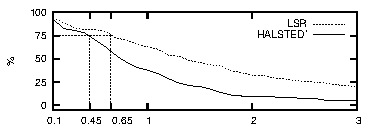
\includegraphics[width=3in]{lsrvscostpd.pdf}

\% false alarms:

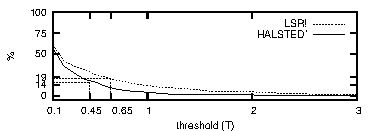
\includegraphics[width=3in]{lsrvscostpf.pdf}
\end{center}}
\caption{
 Y-axis shows probability of false alarm,
  and
  probability of recognizing defective modules  seen using \mbox{$d_i \ge T$}.
  Curves calculated from the KC2 dataset from the PROMISE repository goo.gl/pGDfvp.
 }\label{fig:pd1}
 \end{figure}


One   lesson from  \fig{pd1} is that the ``best'' tunings are context
specific. For mission critical systems (e.g. a nuclear power plant), management
might accept the cost of high false alarm rates if it meant increasing the probability
of detecting errors. For such contexts, we might recommend some very small value of $T$.

The other   lesson from   \fig{pd1}  is that, with tuning, a seemingly poor
detector can work just as well as seemingly better ones.
Note that either the Halstead or LOC detector can reach some desired
level of recall, regardless of their correlations, just by
selecting the appropriate threshold value. For example, in \fig{pd1}, see the recall=75\% values
found at {\em either} $d_i\ge 0.65$ or $d_2\ge 0.45$ (and at the threshold, the false alarm rates
were very similar: 14\% and 19\%).

The  point here is that   the true value of a detector
could not be assessed {\em without} conducting a  tuning study in the context of some business case (in this case, 
issuing a request to an inspection team to review some module).  
Hence, it is important to explore tuning
so the rest of this paper repeats the analysis of this section, but for 
more complex learners.


\section{Background Notes}
 

\subsection{Defect Prediction}


This section is our standard introduction to defect prediction~\cite{me15:book1},
plus   some new results from Rahman et al.'s   2014 FSE paper~\cite{rahman14:icse}. 
 


\begin{figure*}[!t]
\renewcommand{\baselinestretch}{0.8}\begin{center}
{\scriptsize
\begin{tabular}{c|l|p{4.7in}}
amc & average method complexity & e.g. number of JAVA byte codes\\\hline
avg\_cc & average McCabe & average McCabe's cyclomatic complexity seen
in class\\\hline
ca & afferent couplings & how many other classes use the specific
class. \\\hline
cam & cohesion amongst classes & summation of number of different
types of method parameters in every method divided by a multiplication
of number of different method parameter types in whole class and
number of methods. \\\hline
cbm &coupling between methods &  total number of new/redefined methods
to which all the inherited methods are coupled\\\hline
cbo & coupling between objects & increased when the methods of one
class access services of another.\\\hline
ce & efferent couplings & how many other classes is used by the
specific class. \\\hline
dam & data access & ratio of the number of private (protected)
attributes to the total number of attributes\\\hline
dit & depth of inheritance tree &\\\hline
ic & inheritance coupling &  number of parent classes to which a given
class is coupled (includes counts of methods and variables inherited)
\\\hline
lcom & lack of cohesion in methods &number of pairs of methods that do
not share a reference to an instance variable.\\\hline
locm3 & another lack of cohesion measure & if $m,a$ are  the number of
$methods,attributes$
in a class number and $\mu(a)$  is the number of methods accessing an
attribute, 
then
$lcom3=((\frac{1}{a} \sum_j^a \mu(a_j)) - m)/ (1-m)$.
\\\hline
loc & lines of code &\\\hline
max\_cc & maximum McCabe & maximum McCabe's cyclomatic complexity seen
in class\\\hline
mfa & functional abstraction & number of methods inherited by a class
plus number of methods accessible by member methods of the
class\\\hline
moa &  aggregation &  count of the number of data declarations (class
fields) whose types are user defined classes\\\hline
noc &  number of children &\\\hline
npm & number of public methods & \\\hline
rfc & response for a class &number of  methods invoked in response to
a message to the object.\\\hline
wmc & weighted methods per class &\\\hline
\rowcolor{lightgray}
defect & defect & Boolean: where defects found in post-release bug-tracking systems.
\end{tabular}
}
\end{center}
\caption{OO measures used in our defect data sets.  Last line is
the dependent attribute (whether a defect is reported to  a
post-release bug-tracking system).}\label{fig:ck}
\end{figure*}



Human programmers are clever, but flawed. Coding  adds functionality, but also defects.
Hence, software sometimes crashes (perhaps at the most awkward or dangerous moment) or delivers
the wrong functionality. For a very long list of software-related errors,
see  Peter Neumann's ``Risk Digest'' at catless.ncl.ac.uk/Risks.

Since programming inherently
introduces defects into  programs, is important to thoroughly {\em test} software before it is {\em used}.
Such testing  can be very expensive.
Software assessment budgets are finite
while assessment effectiveness increases 
exponentially with assessment effort.
Lowry et al. warn that  
the state space explosion problem imposes
strict limits on how much a system can be explored
via automatic formal methods~\cite{lowrey98}.
For standard black-box testing methods,
a {\em linear} increase
in the confidence $C$ that we have found all defects
can take {\em exponentially} more effort.
For example, for one-in-a-thousand detects,
moving $C$ from  
90\% to 98\% nearly doubles the number of  tests (2301 to   3910 black box
probes, respectively)\footnote{A randomly selected 
input to a program will find a fault with probability $p$.
After $N$ random black-box tests, the chances of the inputs 
not revealing any fault 
is $(1-p)^N$. Hence, the chances $C$ of seeing the fault is $1-(1-p)^N$
which can be rearranged to 
 $N(C,p)=log(1 -
C)/log(1-p)$. For example, $N(0.90,10^{-3})=2301$.}.

Exponential costs quickly exhaust finite resources.
Standard practice is to apply the best
available assessment methods on the sections of the program that the
best available domain knowledge declares is most critical.  We endorse
this approach.  Clearly, the most critical sections require the best
known assessment methods. However, this focus on certain sections
can blind us to defects in other areas.
Therefore, standard practice should be augmented
with a  {\em
lightweight sampling policy} to explore the rest of the system.  This
sampling policy will always be incomplete.
Nevertheless, it is the recommended option when
resources do not permit a complete assessment of the whole system.

One such lightweight sampling policy is defect predictors learned from static code attributes.
Given software described using (for example) the attributes of \fig{ck}, it is possible
to use standard data mining technology to learn where the probability of software defects is highest.
Such defect predictors learned from
static code attributes are   {\em easy to
use}, {\em widely-used}, and {\em useful} to use.

{\em Easy to use:} Static code attributes can be automatically collected, even for very large systems~\cite{nagappan05}.
Other methods, like  manual code reviews, are far slower and far more labor-intensive.
For example, depending on the review methods, 8 to 20 LOC/minute can be
inspected and this effort repeats for all members of the review team,
which can be as large as four or six people~\cite{me02f}. 

%%%%%%%%%%%%%%%% list of parameters%%%%%%%%%%%%%%%%%%%%%
\renewcommand\arraystretch{1.2}
\begin{figure*}[t!]
\scriptsize
  \centering
	\begin{tabular}{|c|c|c|c|l|}
	\cline{1-5}
	\begin{tabular}[c]{@{}c@{}}Learner \\ Name\end{tabular} & Parameters & Default &\begin{tabular}[c]{@{}c@{}}Tuning\\ Range\end{tabular}& 
\multicolumn{1}{c|}{Description} \\ \hline
	\multirow{8}{*}{\begin{tabular}[c]{@{}c@{}}Where-based\\ Learner\end{tabular}} 
	& threshold & 0.5 &[0.01,1]& The value to determine defective or not .\\ \cline{2-5} 
	& infoPrune & 0.33 &[0.01,1]& The percentage of features to consider  for the best 
split to build CART tree\footnote{Since the Where-based learner will build two trees, the first 
one is for clustering and the second one is building prediction model. we explicitly call Where-
clustering tree and CART tree, respectively}. \\ \cline{2-5} 
	 & min\_sample\_split & 4& [1,10]& The minimum number of samples required to split an internal node of
CART tree. \\ \cline{2-5} 
	 & min\_Size & 0.5 &[0.01,1]& \begin{tabular}[c]{@{}l@{}}Finds min\_sample 
in Where-clustering trees  using  ${n\_samples}^ {min\_Size}$.
\end{tabular} \\ \cline{2-5} 
    & wriggle & 0.2 &[0.01, 1] & The threshold to determine which branch in  Where tree to be pruned\\ \cline{2-5}
	 & depthMin & 2 & [1,6]&The minimum depth of the tree below which no pruning for Where-
clustering tree. \\ \cline{2-5} 
	 & depthMax & 10 &[1,20]& The maximum depth of the Where-clustering tree. \\ \cline{2-5} 
	 & wherePrune & False &T/F& Whether or not to prune the Where-clustering tree. \\ \cline{2-5}
	 & treePrune & True &T/F& Whether or not to prune the classification tree built by CART. \\ \cline{2-5} 
\hline
\multirow{4}{*}{CART} & threshold & 0.5 &[0,1]& The value to determine defective or not. \\ \cline{2-5} 
	 & max\_feature & None &[0.01,1]& The number of features to consider when looking for the best 
split. \\ \cline{2-5} 

	 & min\_sample\_split & 2 &[2,20]& The minimum number of samples required to split an 
internal node. \\ \cline{2-5} 
	 & min\_samples\_leaf & 1 & [1,20]&The minimum number of samples required to be at a leaf 
node. \\ \cline{1-5}  
       \multirow{5}{*}{\begin{tabular}[c]{@{}c@{}}Random \\ Forests\end{tabular}}  & threshold & 0.5 & [0.01,1] & The value to determine defective or not. \\ 
\cline{2-5} 
	 & max\_feature & None &[0.01,1]& The number of features to consider when looking for the best 
split. \\ \cline{2-5} 
	 & max\_leaf\_nodes & None &[1,50]& Grow trees with max\_leaf\_nodes in best-first fashion. \\ \cline{2-5} 
	 & min\_sample\_split & 2 &[2,20]& The minimum number of samples required to split an 
internal node. \\ \cline{2-5} 
	 & min\_samples\_leaf & 1 &[1,20]&The minimum number of samples required to be at a leaf 
node. \\ \cline{2-5} 
	 &  n\_estimators & 100 & [50,150]&The number of trees in the forest.\\ \cline{2-5}
	 \hline

	\end{tabular}
    \caption {List of parameters to be tuned.}
\label{fig:parameters}
\end{figure*}
{\em Widely used:} Many researchers and industrial practitioners  use static attributes to guide software 
quality predictions.
 Defect prediction models have been reported
to have been used at Google~\cite{lewis13}.
Verification and validation (V\&V) textbooks
(\cite{rakitin01}) advise using static code complexity attributes
to decide which modules are worthy of manual inspections.  
For several  years, one of us (Menzies) worked on-site at the NASA software Independent Verification
and Validation facility
and he
knows of several large government software contractors that won't
review software modules {\em unless} tools like McCabe predict that
they are fault prone.  


{\em Useful:}
Defect predictors often  find the location of  70\% (or more)
of the defects in code~\cite{me07b}.
Defect predictors developed at NASA~\cite{me07b} have also been used in software development companies outside the US (in Turkey). When the inspection teams focused on the modules that trigger the defect predictors, they found up to 70\% of the defects using just 40\% of their QA effort (measured in staff hours)~\cite{tosun10}.
A subsequent study on the Turkish software
compared how much code needs to be inspected using
random selection vs. selection via defect
predictors. Using random testing, 87\% of the files
would have to be inspected in order to detect 87\%
of the defects. Further, if the inspection process
was restricted to the 25\% of the files that trigger
the defect predictors, then 88\% of the defects
could be found. That is, the same level of defect
detection (after inspection) can be achieved using
$(87-25)/87=71$\%less effort
\cite{tosun09}.


Defect predicting technology has been
commercialized in many tools including {\it Predictive}~\cite{turner06}, a
 product suite to analyze and predict
defects in software projects. Predictive was observed to
highlight similar issues to those found   with the more expensive tools. Significantly,
Predictive was able to faster process a larger code
base than the more expensive tool~\cite{turner06}.

The success of this method in  predictors in finding bugs is   markedly
higher than other currently-used
industrial
methods such as manual code reviews. For example, 
a  panel at {\em IEEE Metrics
2002}~\cite{shu02} concluded that manual software  reviews can find ${\approx}60\%$ 
of defects.
In other work, 
Raffo documents the typical    defect detection capability of
industrial review methods:   around 50\%
 for full Fagan inspections~\cite{fagan76} to
21\% for less-structured inspections.

Note only do static code defect predictors perform well compared to manual methods,
they also are competititve with certain automatic methods.
At ICSE'14, Rahman et al.~\cite{rahman14:icse} compared:
\bi
\item The static code analysis tools FindBugs, Jlint, and Pmd;
\item Against static code defect predictors
(which they called ``statistical defect prediction'') build using logistic regression.
\ei
They found  no significant differences in the cost-effectiveness
of these  approaches. Given this equivalence, it is significant to note that 
static code defect prediction can be quickly adapted to new languages by building lightweight
parsers that find   information like \fig{ck}. The same is not true for   static code analyzers-- these need  extensive modification before they can be used on new
languages.



 

\subsection{Data Mining Algorithms}
 
Dta miners find generalizations (a.k.a. summaries)
of the data. All such generalizations must be smaller than the data it generalizes (otherwise we might as well just keep the original data and ignore the generalization)\footnote{Technical note:
even instance-based reasoners uses generalizations when they partially match new cases to old;
or if they use some  clustering algorithm to restrict the case matching
to just the subset of old cases most similar  to new  cases.}. 
Generalization is important since,
without generalization, all we can do is perform exact matches
of new situations to a database of old examples. This is not recommended practice since,
 if the new situation has not occurred  before, then nothing in the data  will
 matches the new situation
(and we cannot make any predictions).

The key point here is that there are many ways to summarize data and exceConsider some learner that
builds predictive rules form a subset of  attributes $A$ ranges. Assuming numeric attributes
divided into five ranges, then the 20 attributes of \fig{ck} can be combined into 
$2^{5*20}> 10^{30}$
possible rules 

\section{Algorithm: Predictor and Tuner}

In order to conduct the experiment of this paper, we need one tool that can predict defects 
from the empirical data sets and a second tool to tune the built-in parameters associated with 
predictor. To compare the effects of the tuning process, we have three different predictors: 
WHERE-based Predictor, CART and Random Forest. Different Evolution(DE) as an optimizer 
is used as a tuner in this paper.

We choose CART and Random Forest as a predictor in this paper is motivated by 
\cite{lessmann2008benchmarking}, where the performance of both tools as predictors are 
significantly different based on authors' experiment as mentioned before. We'd like to 
investigate whether tuning can change such conclusion. WHERE-based Predictor is a new 
defect predictor based on WHERE\cite{menzies2013local} algorithm. A comparison with 
standard predictor like CART and Random Forest will better evaluate and judge the 
performance such new predictor. As for the tuner, there're many heuristic optimization 
algorithms in wild. However, DE is a good but maybe not the best candidate for the tuning 
process considering different performance measurements. To determine which optimizer is 
fitable and results in better performance is beyond this work scope. We leave it to future 
works. The rest of this section will describe each tool applied in this work.

 \subsection{WHERE-based Learner}
\textbf{WHERE-based Learner} is composed of WHERE clustering algorithm and CART 
decision tree algorithm. The key idea of WHERE-based learner is that  instead of training the 
CART decision tree based on the class labels associated with each training sample, it's using 
CART to build decision trees based on the cluster labels, which are generated by the WHERE 
clustering algorithm.
 
 
 
\begin{figure}[!t]

\renewcommand{\baselinestretch}{0.8}
\scriptsize
\centering
  \begin{tabular}{r@{~}|r@{~}rr|r@{~}rr|r@{~}rr}
    & \multicolumn{3}{c|}{WHERE}&\multicolumn{3}{c|}{CART}& \multicolumn{3}{c}{Random Forest}\\\cline{2-10} 
    Goal & tuned & naive &$\frac{\mathit{tuned}}{\mathit{naive}}$& tuned & naive &$\frac{\mathit{tuned}}{\mathit{naive}}$& tuned & naive&$\frac{\mathit{tuned}}{\mathit{naive}}$\\\hline
pd&71.4&1.2&60&4.4&0.1&44&7.1&0.2&36\\ 
prec&82.8&1.4&59&3.9&0.1&39&7.4&0.2&37\\
f&86.1&1.2&72&3.3&0.1&33&6.7&0.2&34
  \end{tabular}
  \caption{For one train/test set pair (ANT),  time (in seconds) spent tuning,
  for different goals, or just running the ``off-the-shelf'' learner.}
\end{figure}


\begin{figure}[!t]

\renewcommand{\baselinestretch}{0.8}
\scriptsize
\centering
\begin{tabular}{r|rrr}
goal &	WHERE	&CART&	Random Forest\\\hline
f	&15	&13	&9\\ 
pd	&15	&16	&8\\ 
prec&	14	&14	&8
\end{tabular}
\caption{How much slower is tuning vs just running the default
settings of the learner? E.g. bottom right, tuning to increase
precision with Random Forests is eight times slower than
just running Random Forests.}
\end{figure}



% Given N instances, instead of building decision tree directly with CART, we use WHERE to 
%cluster instances. 
WHERE is a fast clustering algorithm designed by {\it menzies} for finding software artifacts 
with similar attributes. It clusters data on dimensions synthesized along the axis of greatest 
variability in the data. The way WHERE used to find such dimension is a linear-time heuristic 
called ``FASTMAP" proposed by Faloutsos \& Lin\cite{faloutsos1995fastmap}. ``FASTMAP" 
randomly picks one instance $Z$; find the instance {\it east} $X$ that's furthest away form $Z$; find 
the instance {\it west} $Y$ that's furthest away from {\it east} $X$. Next, project all the remaining 
points onto the line drawn between $X$ and $Y$.  The line $\overline{XY}$ is an approximation of the 
first component found by PCA. As shown in Figure \ref{Where}, $X$ and $Y$ are the furthest points found by ``FASTMAP'' and $\overline{XY}$ is of length $c$. Each point in this figure has a distance $a$
to $X$ and distance $b$ to $Y$. According to the coisne rule and Pythagoras, each instance will be mapped 
into 2-dimension by the following equations.
\begin{equation}
\begin{split}
x  &= (a^2 +c^2-b^2)/(2c)\\ 
   y  &= \sqrt{a^2 -x^2}
\end{split}
\end{equation}


Then choose the median point $\hat{x}$ as the split and 
recursively divide all the instances into {\it west} and {\it east} clusters until the number of 
instances within each cluster is less than specific minimum size. The representation of the 
clustering result is a tree, we call it Where-clustering tree. Such tree will be pruned if applicable 
in some cases. Finally, cluster labels  will be assigned to instances in each of those 
clusters(leaves). 

\begin{figure}[!ht]
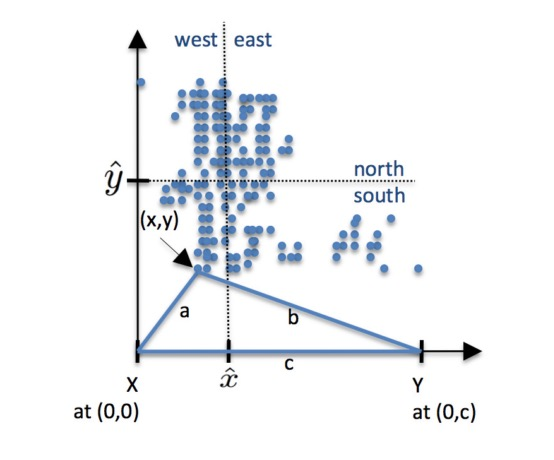
\includegraphics[scale=0.5]{where.png}
\caption{WHERE algoirthm }
\label{Where}
\end{figure}
Then based on the attributes and the cluster labels in each instances,  we build a 
decision tree based on CART algorithm. In each leaf of the tree, there're several instances 
falling in. This will be the model trained for defect prediction. During testing process, a new 
instance comes in and traverses the tree according to 
values of the its attributes. If the instance could reach one leaf of the tree, the predicted value 
of this instance will be the mean  of all the training data values associated with this leaf. 
Otherwise if stops at intermediate nodes of tree, the predicted value will be the mean of the all 
the training data value below this node. After estimating all the number of defectives in the test 
data, whether each instance contains defectives will be determined by comparing with a threshold value. If the predicted value is greater than threshold, the Where-based learner will predict this instance as defective otherwise non-defective.


%\begin{algorithm}
%	\caption{Pesudocode for WHERE Algorithm }
%	\label{alg:WHERE}
%	\begin{algorithmic}[1]
%	\Require $data$
%	\Ensure $tree$
%	\Function {Fastmap}{$ data$}
%	\State $one \gets$ any$(data)$
%	\State $west \gets$ furthest$(data, one)$
%	\State $east \gets$ furthest$(data, west)$
%	\State $c \gets$ distance($west, east$)
%	\EndFunction
%	\end{algorithmic}            
%\end{algorithm}

\subsection{CART}
\textbf{CART} is an {\em iterative dichotomization} algorithm
that finds the attribute that most divides the data such that
the variance of the goal variable in each division is
minimized\cite{breiman84}.
The algorithm then recurses on each division.
Finally, the cost data in the leaf divisions
is averaged to generate the estimate.

\subsection{Random Forests}

Breiman's website describes \textbf{Random Forests} as
follows\cite{brieman00}. "Random Forests grows many classification
trees. To classify a new object from an input vector, put the input
vector down each of the trees in the forest. Each tree gives a
classification, and we say the tree "votes" for that class. The forest
chooses the classification having the most votes (over all the trees
in the forest). Each tree is grown as follows.
If the number of cases in the training set is N, sample N cases at
random - but with replacement, from the original data. This sample
will be the training set for growing the tree.
Also, if there are M input variables, a number m$<<$M is specified such
that at each node, m variables are selected at random out of the M and
the best split on these m is used to split the node. The value of m is
held constant during the forest growing.
Finally, each tree is grown to the largest extent possible (there is
no pruning)."




%Suppose the cordinates of X and Y are $(0,0)$ and $(0,c)$, which are east and west 
%instances within N samples. From the Pythegoras and cosine rule, each instance is projected 
%at the point(x,y)
%
%\begin{equation}
%	\begin{split}
%	x &= (a^2 + c^2 - b^2)/(2c) \\
%	y &= \sqrt{a^2 - x^2} 
%	\end{split}
%\end{equation}

 
 
The psuedocode for differential evolution is shown in Algorithm~\ref{alg:DE}.
Note that, as we describe the algorithm,
  any superscript number denotes a line in that algorithm.


DE is an evolutionary algorithm where next {\em NewGeneration} is learnt from
a current {\em Population}.  If the new is no better than  current, then
we lose one life (terminating when lives is zero)$^5$.

Each candidate solution in the {\em Population}  
is a pair of {\em (Tunings, Scores)}.  {\em Tunings} are selected from
\fig{parameters} and {\em Scores} come from training a learner using those parameters
and applying it     test data$^{23-28}$.

The premise of DE  is that the best way to mutate existing tunings
is to {\em Extrapolate}$^{29}$
between current solutions.  Three solutions $a,b,c$ are selected at random.
For each tuning parameter $i$, at some probability {\em cr}, we replace
the old tuning $x_i$ with $y_i$:
\bi
\item (For numerics) $y_i = a_i+f \times (b_i - c_i)$   where $f$ is a parameter
controlling the cross-over amount.  The {\em trim} function$^{39}$ limits the new
value to the legal range min..max of that parameter.
\item (For booleans) $y_i= \neg x_i$ (see line 37).
\ei
The main loop of DE$^7$ runs over the {\em Population}, replacing old items
with new {\em Candidate}s (if the new candidate is better than the old item).
This means that, as the loop progresses, the {\em Population} is full of increasiningly
more valuable solutions. This, in turn, also improves  the candidates, which are generated
from the {\em Population}.

For the experiments of this paper, we collect performance
values from a data mining, from which a {\em Goal} function extracts one 
performance value$^{27}$ (so we run this code many times, each time with
a different {\em Goal}$^2$).  Technically, this makes a  {\em single objective} DE (and for notes on multi-objective DEs, see~\cite{Coello05,zhang07,5583335}).


%\begin{algorithm}
%\begin{algorithmic}[1]
% \KwData{this text}
% \KwResult{how to write algorithm with \LaTeX2e }
% initialization\;
% \While{not at end of this document}{
%  read current\;
%  \eIf{understand}{
%   go to next section\;
%   current section becomes this one\;
%   }{
%   go back to the beginning of current section\;
%  }
% }
% \caption{How to write algorithms}
% \end{algorithmic}
%\end{algorithm}




\section{Experimental Design}

The following experiment aims to compare the performance of three learners, tuned and untuned, on 17
sets of data. 

\subsection{Data Sets}

Our defect data comes from the PROMISE repository\footnote{http://openscience.us/repo}.
It pertains to 
open source Java systems defined in terms of \fig{ck}:  {\it ant}, {\it camel}, {\it ivy}, {\it jedit}, {\it log4j}, {\it lucene},
{\it poi},{\it synapse}, {\it velocity} and {\it xerces}. 

An important principle in data mining is not to test on the data used
in training.  There are many ways to design a experiment that satisfies this principle.
Some of those methods have  limitations:
\bi
\item  Leave-one-out is too slow for large data sets;
\item Cross-validation can mix up older and newer data sets so it may well be that
data from the {\em future} is used to test on {\em past data}.
\ei
To avoid these problems, we used an incremental learning approach. The following
experiment ensures that the training data was created at some time before the test
data.

For this experiment, we use data sets with at least three  
consecutive releases  (where release $i+1$ was built after release $i$).
\bi 
\item The {\em first} release was used for some  {\em training}, to collect a baseline
   using an untuned learner. This release is also used  on line 24 of Algorithm~\ref{alg:DE} to
   build some model using some the tunings found in some {\em Candidate}.
   \item The {\em second} release was used on 25 of Algorithm~\ref{alg:DE} to 
   test the model found on line 24.
   \item Finally the {\em third} release was used to gather the performance statistics
   reported below from (a)~the model generated by the untuned learner or (b)~the
   best model found by differential evolution.
   \ei
This approach ensures   all treatments 
are assessed on the same tests.

Some data sets have more than three releases and, for those data, we could run more
 than one experiment. For example, {\em ant} has five versions in PROMISE so
 we ran three experiments called V0,V1,V2:
 \bi
 \item AntV0: first,second,third = versions 1,2,3
 \item AntV1: first,second,third = versions 2,3,4
 \item AntV2: first,second,third = versions 3,4,5
 \ei 
These data sets are displayed in \fig{data1}.


\begin{figure}[!b]
\small
\begin{tabular}{|p{.95\linewidth}|}\hline
One style
of measure is to check the {\em variability} of that predictor.
For example,
in their study on reproducibility of SE results,
 Anda, Sjoberg and Mockus advocate using the coefficient of variation ($CV=\frac{stddev}{mean}$).
Using this measure, they defined {\em reproducibility} as $\frac{1}{CV}$~\cite{anda09}.

There exist other goals that combine defect prediction with other economic
factors.
Arisholm~\&~Briand~\cite{arisholm06},  Ostrand \& Weyeuker~\cite{ostrand04} and Rahman et al.~\cite{rahman12}
say that a defect predictor should maximizing {\em reward}; i.e. find the fewest lines of code
that contain the most bugs.

Yin et al. are concerned about
 {\em incorrect bug fixes}; i.e. those that require subsequent work in order to complete the bug fix.
These bugs occur  when (say) developers try to fix parts of the code
where they have very little experience~\cite{yin11}.  To avoid such incorrect bug fixes, we have to optimize
for finding the most number of bugs in regions that {\em the most programmers have worked with before}.

In {\em Better-faster-cheaper},   project want changes that lead
to fewer defects,  faster development,  using less resources~\cite{Green,elrawas08,elrawas10,me07f,me09a,me09f}.

Another  {\em  rush-to-market} approach is yet another economic-based optimization measure.
A learner that tries to maximize ``rush-to-market'' is trying to release the product as soon
as possible, without too many bugs. Note that ``rush-to-market'' is an appropriate strategy for a company competing
in a volatile and crowded market place where being first-to-market enables a revenue stream (that can be
used to subsequently fix any issues with version 1.0)~\cite{huang06}.\\\hline
\end{tabular}
\caption{Many ways to assess defect predictors.}\label{fig:criteria}
\end{figure}
 \begin{figure*}[!t]

\renewcommand{\baselinestretch}{0.8}
\scriptsize
\centering
  \begin{tabular}{c c c c c c c c c c }\hline
  Dataset &antV0&antV1&antV2&camelV0&camelV1&ivy&jeditV0&jeditV1&jeditV2
\\\hline
  training &20/125 &40/178 &32/293 &13/339 &216/608 &63/111 &90/272 &75/306 &79/312
\\  tuning  &40/178 &32/293 &92/351 &216/608 &145/872 &16/241 &75/306 &79/312 &48/367
\\  testing &32/293 &92/351 &166/745 &145/872 &188/965 &40/352 &79/312 &48/367 &11/492
\\ \hline
  Dataset &log4j&lucene&poiV0&poiV1&synapse&velocity&xercesV0&xercesV1
\\\hline
  training &34/135 &91/195 &141/237 &37/314 &16/157 &147/196 &77/162 &71/440
\\  tuning  &37/109 &144/247 &37/314 &248/385 &60/222 &142/214 &71/440 &69/453
\\  testing &189/205 &203/340 &248/385 &281/442 &86/256 &78/229 &69/453 &437/588
\\  \end{tabular}

   \caption{Ratios of defective instances in each experimental data set. 
   E.g., the top left data set has 20 defective classes out of 125 total.
   This paper runs one experiment for each column
   shown in this figure. The {\em training} set is used by an untuned learner
   to build a model, which is then tested on the {\em testing} data.
   {\em Training} data is used by  differential evolution when it builds
    a model (using one set of possible tunings) and that model is tested on {\em tuning} data.
    Finally, the best model from by DE is applied to {\em testing}.  
   }\label{fig:data1}
\end{figure*} 

\subsection{Optimization Goals}

Recall from Algorithm~1 that we call differential evolution once for each
 optimization goal. This section lists those optimization goals.

Let $\{A,B,C,D\}$ denote the
true negatives, 
false negatives, 
false positives, and 
true positives
(respectively) found by a binary detector. 
Certain standard measures can be computed from
$A,B,C,D$: 

{\scriptsize\[
\begin{array}{ll}
pd=recall=&D/(B+D)\\
pf=&C/(A+C)\\
pf'=& 1 - pf\\
prec=precision=&D/(D+C) 
\end{array}
\]}

All the above vary from zero to one. For $pf$, the {\em better} scores are {\em smaller}.
For all other scores, the {\em better} scores are {\em larger}.

The following results make no assumption that (e.g.) minimizing false alarms is 
more important than maximizing   precision. That determination 
depends on current business conditions:
\be
\item
For safety critical applications, high false alarm rates may be acceptable if the cost
of overlooking any critical can outweigh the inconvenience of having to inspect a few more
modules. 
\item
On the other hand, when rushing a product to market before a competing product is released, there is a business case to 
avoid the extra rework associated with false alarms.  In that business context, 
managers might be willing to lower the recall somewhat in order to minimize the false alarms.
\ee
These two examples are just the tip of the iceberg (see other criteria in \fig{criteria})
and there is insufficient space in this paper to explore all the above optimization goals.
What we can do, however, is show examples of how  changing  optimization goals can also change 
the conclusions made from that learner on that data. Those examples only relate to precision, recall, and the F-measure
but the general principle (that the search bias changes the search conclusions) would hold for all the goals
listed in the previous paragraph.  Hence, we warn that it is important not to overstate  empirical results from software analytics.
Rather, those results need to be expressed {\em along with} the context within which they are
relevant (and by ``context'', we mean the optimization goal).


\section{Experimental Results}

The introduction of this article made several claims about tuning defect predictor
that use static code attributes. This section presents
support for those claims:
\be
\item  Tuning    improves the performance scores of a predictor;
e.g.  precision changes from 2\% to 98\%: see \tion{precision};
\item Tuning changes conclusions on what learners are better than others: see \tion{rank};
\item Tuning changes conclusions about what factors are most important: see \tion{import};
\item  Tuning is easy: see \tion{easy};
\item Tuning is fast: see \tion{fast};
\item Data miners should not be used ``off-the-shelf'' with their default tunings: see \tion{variance}.
\ee


One comment before continuing. The following text does not
show results for tuning on recall
or false alarms. The reason is that false alarm and recall focus on {\em only}
the non-defective and defective modules (respectively). Hence:
\bi
\item
When DE tunes for recall, we can achieve near
100\% recall-- but the cost of a near 100\% false alarms.
\item
Similarly, the tuner
could achieve near zero false alarm rates by effectively turning off
the detector (driving recall to zero).
\ei
Hence, in the
following, we explore performance measures that comment on all the possible
target classes (i.e. precision and ``F''). 

\subsection{Tuning Can  Improves Performance Scores}\label{sect:precision}

\fig{precisionbars} shows precision results before and after tuning using three different learners.
For each data set, the maximum precision values for each data set are shown in {\bf bold}.


These results offer support for the prior conclusions of  
 Lessmann et al.~\cite{lessmann2008benchmarking} (that CART is worse than Random Forest):
\bi
\item
Untuned CART is indeed the worst learner (none of its
untuned results are best and {\bf bold}). 
\item 
In $\frac{15}{17}$ cases, untuned Random Forest out-performs  untuned CART.  
\ei
Some of the data sets in \fig{precisionbars} proved challenging for all learners;
e.g. the precision results for {\em ivy} are less
that impressive.
To some extent, this can be explained by
the properties of of the data set (as shown in \fig{data1}, defective classes in {\em ivy} are very rare in tuning data).

That said,  tuning can improve those poor performing detectors:
\bi
\item
For {\em xercesV0}, nearly all learners report precisions of under 20\%. But tuned  WHERE scores a 85\% precision.  
\item A similar pattern can be seen in results from {\em camelV0},   and {\em jeditV2}.
In those two data sets, nearly all the precision values are   low {\em except} for
tuned WHERE that scored 83\% and 98\%.
\ei
Finally, note the  {\em jeditV2} result for the WHERE learner.
Here, tuning changes precision from 2\% to 98\%.

\fig{deltas} shows that tuning usually has a positive effect on performance scores. This figure sorts
the deltas in the precision and the F-measure    between tuned and untuned learners. Our reading of this
figure is that, overall, tuning rarely makes performance   worse and usually can make it much better. 
 


\begin{figure}[!t]
\renewcommand{\baselinestretch}{0.8} 

\scriptsize    

\begin{tabular}{r|rl|rl|rl|rl|rl|rlrl}
%\begin{tabular}{r@{~}|r@{~}l@{~}|r@{~}l@{~}|r@{~}l|r@{~}l@{~}|r@{~}l@{~}|r@{~}l@{~}r@{~}l}
      &   \multicolumn{4}{c|}{WHERE}         &   \multicolumn{4}{c|}{CART}         &   \multicolumn{4}{c}{Random Forest}         \\\hline
  Data set   &   \multicolumn{2}{c}{default}         &   \multicolumn{2}{c|}{Tuned}         &   \multicolumn{2}{c}{default}         &   \multicolumn{2}{c|}{Tuned}    &   \multicolumn{2}{c}{default}  &   \multicolumn{2}{c}{Tuned}\\\hline
antV0 & 30 &         & {\bf 89} & {\rfour} & 27 &         & {\bf 89} & {\rfour} & 39 &         & {\bf 89 }& {\rfour}\\
antV1 & 32 & {\rtwo} & {\bf 74} & {\rfour} & 41 & {\rtwo} & {\bf 74 }& {\rfour} & 43 & {\rtwo} & 0 &        \\
antV2 & {\bf 78} & {\rfour} & {\bf 78} & {\rfour} & 52 &         & 68 & {\rthree} & 66 & {\rtwo} & 67 & {\rtwo}\\
camelV0 & {\bf 83} & {\rfour} & {\bf 83} & {\rfour} & 26 &         & 33 &         & 34 &         & 45 & {\rone}\\
camelV1 & 22 &         & {\bf 28} & {\rfour} & 23 &         & 24 & {\rone} & {\bf 28} & {\rfour} & {\bf 28} & {\rfour}\\
ivy & 16 &         & {\bf 23} & {\rfour} & 18 & {\rone} & 21 & {\rthree} & 21 & {\rthree} & 20 & {\rtwo}\\
jeditV0 & 35 &         & {\bf 75} & {\rfour} & 49 & {\rone} & 56 & {\rtwo} & 50 & {\rone} & 48 & {\rone}\\
jeditV1 & 24 &         & {\bf 87} & {\rfour} & 28 &         & 86 & {\rfour} & 36 &         & 39 & {\rone}\\
jeditV2 & 2 &         & {\bf 98 }& {\rfour} & 3 &         & 18 &         & 5 &         & 5 &        \\
log4j & 94 &         & {\bf 100} & {\rfour} & 97 & {\rtwo} & {\bf 100} & {\rfour} & {\bf 100} & {\rfour} & {\bf 100 }& {\rfour}\\
lucene & 61 &         & 74 & {\rfour} & 67 & {\rone} & 70 & {\rtwo} & 72 & {\rthree} & {\bf 77} & {\rfour}\\
poiV0 & 70 &         & 68 &         & 77 & {\rfour} & 72 & {\rone} & {\bf 79} & {\rfour} & 76 & {\rthree}\\
poiV1 & {\bf  100} & {\rfour} & 90 & {\rthree} & 73 &         & 89 & {\rtwo} & 81 & {\rone} & {\bf 100} & {\rfour}\\
synapse & 66 &         & 66 &         & 71 & {\rone} & {\bf 100} & {\rfour} & 59 &         & 80 & {\rtwo}\\
velocity & 34 &         & 39 & {\rthree} & 34 &         & 40 & {\rfour} & 40 & {\rfour} & {\bf 41} & {\rfour}\\
xercesV0 & 13 &         & {\bf 85} & {\rfour} & 14 &         & 13 &         & 15 &         & 13 &        \\
xercesV1 & {\bf 56} & {\rfour} & 26 &         & 50 & {\rthree} & 26 &         & 41 & {\rtwo} & 26 &        \\
\end{tabular}
\caption{Precision results (best results  shown in {\bf bold}).}
\label{fig:precisionbars}
\end{figure}

\begin{figure}[!b]
\begin{center}
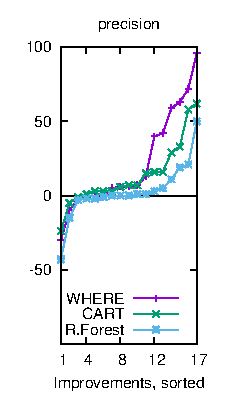
\includegraphics[width=1.25in]{precision1.pdf}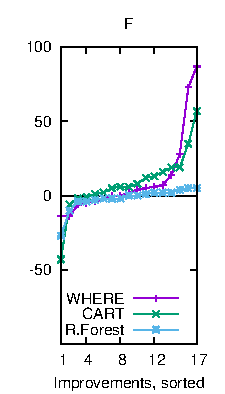
\includegraphics[width=1.25in]{F1.pdf}
 \end{center}
\caption{Deltas in performance  seen in \fig{precisionbars} (left)
and \fig{fbars} (right) between tuned and untuned learners. Tuning improves performance when the deltas are above zero.}\label{fig:deltas}
 \end{figure}

\subsection{Tuning Changes Learner Rankings}\label{sect:rank}
Researchers often use performance criteria to assert that one learner is better than another~\cite{lessmann2008benchmarking,hall11,me07b}.
Such conclusions are   not reliable since they can change when we elect to tune for different goals. 

For example, given the poor showing of untuned CART and the good performance of tuned WHERE
in   \fig{precisionbars}, we might recommend
{\em not} to use CART and {\em always} used tuned WHERE. In turns out that this
conclusion is not stable across the tuning process.


\fig{fbars} shows what happens when we tune for the f-measure. 
As before, untuned Random Forest generally beats CART. However:
\bi
\item
In  a result that is the direct opposite of   
 Lessmann et al.~\cite{lessmann2008benchmarking}, tuned CART does better than Random Forest;
 \item 
 In another result that is the reverse of \fig{precisionbars}, tuned WHERE is not necessarily
 any better than anything else.
 \ei
The lesson here is that, given a particular task (e.g. optimizing for precision), tuning can offer
substantial benefits. However, when that task changes (e.g. to optimizing for the F-measure),
it should not be assumed that conclusions from the previous tuning will hold in the new context.
In practice, this means that tuning needs to be repeated for each new context.





\begin{figure}[!t]
\renewcommand{\baselinestretch}{0.8} 

\scriptsize  
~~~\begin{tabular}{r|rl|rl|rl|rl|rl|rlrl}
      &   \multicolumn{4}{c|}{WHERE}         &   \multicolumn{4}{c|}{CART}         &   \multicolumn{4}{c}{Random Forest}         \\\hline
  Data set   &   \multicolumn{2}{c}{default}         &   \multicolumn{2}{c|}{Tuned}         &   \multicolumn{2}{c}{default}         &   \multicolumn{2}{c|}{Tuned}    &   \multicolumn{2}{c}{default}  &   \multicolumn{2}{c}{Tuned}\\\hline
antV0 & {\bf 39} & {\rfour} & 25 & {\rtwo} & 32 & {\rthree} & 31 & {\rthree} & {\bf 39} & {\rfour} & 12 &        \\
antV1 & 11 &         & 6 &         & 40 & {\rfour} & {\bf 45} & {\rfour} & 39 & {\rfour} & 44 & {\rfour}\\
antV2 & 0 &         & {\bf 87} & {\rfour} & 44 & {\rtwo} & 1 &         & 50 & {\rtwo} & 51 & {\rtwo}\\
camelV0 & 0 &         & 28 & {\rfour} & 9 & {\rone} & 28 & {\rfour} & {\bf 34} & {\rfour} & 30 & {\rfour}\\
camelV1 & {\bf 34} & {\rfour} & {\bf 34} & {\rfour} & 31 &         & 32 & {\rone} & 33 & {\rthree} & 31 &        \\
ivy & 27 &         & 34 & {\rthree} & 30 & {\rone} & {\bf 38} & {\rfour} & 35 & {\rthree} & 33 & {\rtwo}\\
jeditV0 & 50 &         & 56 & {\rtwo} & 56 & {\rtwo} & 54 & {\rone} & {\bf 61} & {\rfour} & 59 & {\rfour}\\
jeditV1 & 37 & {\rone} & 33 &         & 36 &         & {\bf 49} & {\rfour} & 45 & {\rthree} & 47 & {\rfour}\\
jeditV2 & 4 &         & 8 & {\rtwo} & 5 &         & {\bf 11} & {\rfour} & 9 & {\rthree} & 9 & {\rthree}\\
log4j & {\bf 62} & {\rfour} & 56 & {\rthree} & 47 & {\rone} & 59 & {\rfour} & 53 & {\rtwo} & 43 &        \\
lucene & 70 & {\rthree} & {\bf 75} & {\rfour} & 56 &         & {\bf 75} & {\rfour} & 73 & {\rfour} & {\bf 75} & {\rfour}\\
poiV0 & {\bf 78} & {\rfour} & 64 &         & 74 & {\rthree} & 68 & {\rone} & 73 & {\rthree} & 69 & {\rone}\\
poiV1 & 5 &         & {\bf 78} & {\rfour} & 21 & {\rone} & {\bf 78} & {\rfour} & 76 & {\rfour} & {\bf 78} & {\rfour}\\
synapse & 0 &         & 2 &         & 40 & {\rthree} & {\bf 56} & {\rfour} & 51 & {\rfour} & 55 & {\rfour}\\
velocity & {\bf 51} & {\rfour} & {\bf 51} & {\rfour} & 49 &         & {\bf 51} & {\rfour} & {\bf 51} & {\rfour} & {\bf 51} & {\rfour}\\
xercesV0 & 22 & {\rone} & 20 &         & 21 &         & {\bf 27} & {\rfour} & 23 & {\rtwo} & 20 &        \\
xercesV1 & 25 &         & 39 & {\rone} & 18 &         & 53 & {\rthree} & 68 & {\rfour} & {\bf 73} & {\rfour}\\
\end{tabular}
\caption{F-value results (best results  shown in {\bf bold}).}
\label{fig:fbars}
\end{figure}


\subsection{Tuning Changes Factors Rankings }\label{sect:import}


Researchers often use data miners to  test what factors have most impact on software projects~\cite{bell2013limited,rahman2013how,me02k,moser2008comparative,zimmermann2007predicting,herzig2013predicting}. 
As above, we can show that such conclusions are not reliable since they can be changed by tuning.

\fig{counts} shows how the objective goal (in this case,
 precision or the f-measure) changed what attributes were used
in the decision tree learners
(in this case, WHERE building trees to select for different clusters). 


Note that the counts in the {\em tuned} column are   usually
different to those in the {\em default} columns (the tuned learners used more attributes
than otherwise as witnessed by the taller columns of numbers in the ``tuned'' column).




\subsection{Tuning is Easy}\label{sect:easy}

In terms of the search space
explored via tuning, optimizing defect prediction from static code
measures is much {\em smaller} than standard optimization.

To see this,
recall from Algorithm~1 that
DE explores a {\em Population} of size {\em np=10}. This is a very small population size since
Rainer Storn (one of the inventors of DE) recommends  setting {\em np} to be ten times larger than the number
of attributes being optimized~\cite{storn1997differential}.

From \fig{parameters},
we see that Storn would therefore recommend {\em np} values of
90, 50, 60 for WHERE, CART and Random Forests (respectively). Yet we achieve our results
using a constant {\em np=10}; i.e. $\frac{10}{90}, \frac{10}{50}, \frac{10}{60}$ of the
recommended search space.

Another measure showing that tuning is easy 
(for static code defect predictors)
is the number of evaluations required to complete optimization
(see next section).



\begin{figure}[!t]

\renewcommand{\baselinestretch}{0.8}
\scriptsize
\centering
  \begin{tabular}{c|c c|c c|c c|c c| c c }
  
    &   \multicolumn{2}{c|}{Precision} & \multicolumn{2}{c|}{F} &  \multicolumn{2}{c|}{SUM}\\
 &&&&&&&\\
Features&   
  default
& tuned
& default
& tuned
& default
& tuned
\\\hline

noc &		  &    &    &   \\
ca  &    &    &    &    &    &\\   
max\_cc  &    &  1  &    &  1  &    &  2\\
ce  &    &  1  &    &  2  &    &  3\\
moa  &    &  1  &    &  2  &    &  3\\
cbo  &    &  1  &    &  4  &    &  5\\
avg\_cc  &    &  3  &    &  2  &    &  5\\
lcom  &    &  3  &    &  3  &    &  6\\
npm  &    &  5  &    &  4  &    &  9\\
cbm  &  6  &  3  &  4  &  3  &  10  &  6\\
amc  &  4  &  3  &  4  &  5  &  8  &  8\\
rfc  &  4  &  5  &  4  &  9  &  8  &  14\\
ic  &  7  &  4  &  9  &  4  &  16  &  8\\
wmc  &  5  &  6  &  5  &  11  &  10  &  17\\
dit  &  8  &  6  &  8  &  6  &  16  &  12\\
lcom3  &  9  &  7  &  9  &  7  &  18  &  14\\
loc  &  8  &  6  &  9  &  12  &  17  &  18\\
cam  &  9  &  8  &  9  &  10  &  18  &  18\\
dam  &  14  &  9  &  14  &  11  &  28  &  20\\
mfa  &  16  &  11  &  16  &  13  &  32  &  24
 
  \end{tabular}
    \caption{Counts of features selected by different goals.Given that we are processing 17 data sets, the maximum counts for any 
one cell in the ``precision'' or ``F'' column is 17.  
    }\label{fig:counts}
\end{figure}
 

\begin{figure*}[!ht]

\renewcommand{\baselinestretch}{0.8}
\scriptsize
\centering
  \begin{tabular}{r|c |c |c |c |c |c }
    \hline\hline
    Datasets & Tuned\_Where & Default\_Where & Tuned\_CART & Default\_CART & Tuned\_RanFst & Default\_RanFst\\
    \hline
    antV0 & 50 /  77.16 & 1.30 & 60 /  3.47 & 0.07 & 50 /  6.54 & 0.14\\
    antV1 & 50 /  135.16 & 2.33 & 60 /  4.84 & 0.08 & 50 /  8.61 & 0.19\\
    antV2 & 50 /  368.50 & 6.23 & 60 /  6.67 & 0.14 & 50 /  11.75 & 0.40\\
    camelV0 & 50 /  479.03 & 8.25 & 60 /  11.73 & 0.18 & 60 /  15.69 & 0.31\\
    camelV1 & 60 /  1551.51 & 26.87 & 60 /  18.47 & 0.28 & 80 /  37.96 & 0.73\\
    ivy & 80 /  83.80 & 1.01 & 50 /  3.07 & 0.07 & 60 /  7.63 & 0.17\\
    jeditV0 & 60 /  349.99 & 5.95 & 70 /  8.33 & 0.11 & 50 /  13.40 & 0.30\\
    jeditV1 & 50 /  442.35 & 7.48 & 70 /  8.63 & 0.11 & 70 /  15.52 & 0.37\\
    jeditV2 & 50 /  360.04 & 7.90 & 60 /  8.63 & 0.12 & 60 /  14.33 & 0.38\\
    log4j & 60 /  97.23 & 1.49 & 70 /  3.31 & 0.06 & 80 /  8.79 & 0.17\\
    lucene & 70 /  206.41 & 2.89 & 80 /  6.90 & 0.08 & 60 /  10.30 & 0.25\\
    poiV0 & 70 /  338.44 & 4.28 & 60 /  6.47 & 0.13 & 60 /  12.45 & 0.29\\
    poiV1 & 60 /  468.73 & 7.95 & 50 /  7.24 & 0.14 & 70 /  17.66 & 0.30\\
    synapse & 50 /  111.30 & 1.87 & 60 /  3.85 & 0.05 & 60 /  7.82 & 0.15\\
    velocity & 60 /  192.83 & 2.66 & 90 /  6.11 & 0.06 & 80 /  12.99 & 0.22\\
    xercesV0 & 70 /  139.33 & 2.23 & 60 /  6.47 & 0.11 & 50 /  8.89 & 0.25\\
    xercesV1 & 50 /  759.82 & 13.11 & 50 /  8.62 & 0.14 & 60 /  16.90 & 0.37\\
  \end{tabular}
  \caption{Evaluations/runtimes  (in seconds), optimizing for  precision.  }\label{fig:etimes}
\end{figure*}


%%%%time for F %%%%%%
\begin{figure*}[!ht]
\renewcommand{\baselinestretch}{0.8}
\scriptsize
\centering
  \begin{tabular}{r|c |c |c |c |c |c }
    \hline\hline
    Datasets & Tuned\_Where & Default\_Where & Tuned\_CART & Default\_CART & Tuned\_RanFst & Default\_RanFst\\
    \hline
    antV0 & 70 / 95.34 & 1.18 & 50 / 3.09 & 0.06 & 60 / 6.89 & 0.13\\
    antV1 & 50 / 130.69 & 2.24 & 50 / 4.47 & 0.08 & 60 / 9.03 & 0.19\\
    antV2 & 50 / 296.68 & 6.66 & 60 / 7.29 & 0.15 & 60 / 12.74 & 0.31\\
    camelV0 & 60 / 496.70 & 8.01 & 60 / 10.43 & 0.17 & 70 / 17.32 & 0.30\\
    camelV1 & 70 / 1732.99 & 23.35 & 60 / 15.93 & 0.22 & 60 / 24.71 & 0.71\\
    ivy & 70 / 58.81 & 1.03 & 70 / 4.07 & 0.06 & 60 / 7.37 & 0.16\\
    jeditV0 & 90 / 412.23 & 5.17 & 70 / 6.59 & 0.08 & 60 / 10.56 & 0.28\\
    jeditV1 & 70 / 425.18 & 6.61 & 60 / 6.15 & 0.10 & 60 / 13.00 & 0.31\\
    jeditV2 & 60 / 398.86 & 6.97 & 50 / 5.90 & 0.12 & 60 / 13.63 & 0.35\\
    log4j & 50 / 68.17 & 1.37 & 60 / 2.46 & 0.04 & 70 / 6.37 & 0.15\\
    lucene & 50 / 147.78 & 2.74 & 50 / 3.79 & 0.07 & 60 / 7.98 & 0.24\\
    poiV0 & 60 / 251.48 & 3.90 & 60 / 5.65 & 0.09 & 70 / 11.25 & 0.30\\
    poiV1 & 60 / 404.96 & 7.22 & 70 / 8.10 & 0.11 & 60 / 12.74 & 0.28\\
    synapse & 50 / 95.37 & 1.80 & 60 / 3.69 & 0.06 & 60 / 7.65 & 0.14\\
    velocity & 60 / 176.80 & 3.40 & 50 / 4.14 & 0.07 & 50 / 7.36 & 0.23\\
    xercesV0 & 60 / 177.48 & 2.34 & 50 / 6.53 & 0.09 & 50 / 14.91 & 0.33\\
    xercesV1 & 50 / 762.28 & 13.33 & 70/ 12.84 & 0.15 & 60/ 16.63 & 0.40\\
  \end{tabular}
  \caption{Evaluations/runtimes  (in seconds), optimizing for  ``F''.  }\label{fig:ftimes}
\end{figure*}


 
%%%%parameters for prec %%%%%%
\begin{figure*}[!ht]
 
\renewcommand{\baselinestretch}{0.9}
\resizebox{\textwidth}{!}{
\scriptsize
\centering
  \begin{tabular}{|c |c |c |c |c |c |c |c |c |c |c |c |c |c |c |c |c |c |c |c |}
    \hline
  \begin{tabular}[c]{@{}c@{}}Learner \\ Name\end{tabular}&Parameters  & Default &antV0&antV1&antV2&camelV0&camelV1&ivy&jeditV0&jeditV1&jeditV2&log4j&lucene&poiV0&poiV1&synapse&velocity&xercesV0&xercesV1\\ 
 \hline
\multirow{8}{*}{\begin{tabular}[c]{@{}c@{}}Where\\based\\ Learner\end{tabular}}
& threshold& 0.5& 0.53& 0.57& 0.14& 0.67& 0.9& 1& 1& 0.72& 0.91& 0.96& 0.67& 1.0& 0.41& 0.24& 1& 0.47& 0.74\\ \cline{2-20}
& infoPrune& 0.33& 0.68& 0.45& 0.53& 0.26& 0.81& 0.42& 0.39& 0.21& 0.05& 0.57& 0.35& 0.53& 0.68& 0.52& 0.56& 0.5& 0.75\\ \cline{2-20}
& min\_sample\_split& 4& 3& 9& 9& 8& 6& 5& 2& 8& 6& 1& 3& 7& 1& 4& 6& 9& 7\\ \cline{2-20}
& min\_Size& 0.5& 0.07& 0.26& 0.39& 0.73& 0.29& 0.49& 0.19& 0.44& 0.36& 1.0& 0.93& 0.45& 0.52& 0.22& 0.91& 0.19& 0.87\\ \cline{2-20}
& wriggle& 0.2& 0.91& 0.63& 0.31& 0.18& 0.97& 0.74& 0.98& 0.59& 0.61& 0.34& 0.92& 0.71& 1& 0.95& 0.25& 0.01& 0.17\\ \cline{2-20}
& depthMin& 2& 4& 5& 1& 5& 3& 1& 4& 1& 3& 3& 1& 3& 1& 2& 5& 3& 2\\ \cline{2-20}
& depthMax& 10& 10& 17& 6& 6& 12& 19& 14& 15& 12& 12& 18& 19& 11& 8& 10& 11& 18\\ \cline{2-20}
& wherePrune& False& True& True& True& False& True& True& True& True& False& False& True& True& True& True& False& True& True\\ \cline{2-20}
& treePrune& True& True& True& False& False& False& True& True& False& False& False& False& False& True& False& False& True& False\\ \cline{2-20}
\hline
\multirow{4}{*}{CART}
& threshold& 0.5& 0.83& 1& 0.99& 0.85& 0.9& 0.93& 1& 0.98& 0.88& 0.9& 0.7& 1& 0.63& 1& 1& 0.91& 0.81\\ \cline{2-20}
& max\_feature& None& 0.01& 0.35& 0.35& 0.73& 0.63& 0.76& 0.76& 0.01& 0.13& 0.01& 0.83& 0.01& 0.02& 0.19& 0.28& 0.97& 0.1\\ \cline{2-20}
& min\_samples\_split& 2& 18& 11& 6& 18& 20& 19& 3& 6& 14& 12& 8& 12& 17& 2& 11& 5& 16\\ \cline{2-20}
& min\_samples\_leaf& 1& 3& 19& 6& 1& 4& 2& 14& 1& 2& 6& 2& 19& 4& 6& 15& 1& 17\\ \cline{2-20}
\hline
\multirow{6}{*}{\begin{tabular}[c]{@{}c@{}}Random \\ Forests\end{tabular}} 
& threshold& 0.5& 0.86& 0.61& 0.71& 0.17& 1& 1& 0.87& 1& 1& 1& 0.97& 1& 0.41& 0.33& 1& 0.83& 0.94\\ \cline{2-20}
& max\_feature& None& 0.05& 0.34& 0.31& 0.45& 0.54& 0.94& 0.93& 0.81& 0.01& 1& 0.69& 0.42& 1& 0.01& 0.01& 0.75& 1\\ \cline{2-20}
& max\_leaf\_nodes& None& 16& 11& 38& 47& 18& 38& 27& 33& 16& 24& 41& 50& 15& 15& 30& 47& 28\\ \cline{2-20}
& min\_samples\_split& 2& 3& 3& 4& 19& 17& 19& 18& 5& 13& 19& 1& 5& 2& 6& 7& 11& 11\\ \cline{2-20}
& min\_samples\_leaf& 1& 7& 11& 10& 16& 8& 14& 4& 2& 7& 14& 12& 7& 10& 12& 7& 8& 4\\ \cline{2-20}
& n\_estimators& 100& 85& 111& 99& 121& 128& 140& 141& 63& 100& 69& 99& 109& 123& 88& 125& 107& 131\\ \cline{2-20}
\hline  \end{tabular}
}
  \caption{Parameters tuned on different models over the objective of precision.}\label{fig:preselect}
\end{figure*}


%%%%parameters for F %%%%%%
\begin{figure*}[!ht]
 
\resizebox{\textwidth}{!}{
\renewcommand{\baselinestretch}{0.9}
\scriptsize
\centering
  \begin{tabular}{|c |c |c |c |c |c |c |c |c |c |c |c |c |c |c |c |c |c |c |c |}
    \hline
    
  \begin{tabular}[c]{@{}c@{}}Learner \\ Name\end{tabular}&Parameters  & Default &antV0&antV1&antV2&camelV0&camelV1&ivy&jeditV0&jeditV1&jeditV2&log4j&lucene&poiV0&poiV1&synapse&velocity&xercesV0&xercesV1\\ 
 \hline
\multirow{8}{*}{\begin{tabular}[c]{@{}c@{}}Where\\based\\ Learner\end{tabular}}
& threshold& 0.5& 0.02& 0.72& 0.97& 0.01& 0.87& 1& 0.59& 0.49& 0.77& 0.38& 0.25& 0.94& 0.01& 0.81& 0.53& 0.83& 0.99\\ \cline{2-20}
& infoPrune& 0.33& 0.13& 0.64& 0.57& 0.33& 0.92& 0.37& 0.43& 0.53& 0.68& 0.56& 0.55& 0.74& 0.04& 0.34& 0.62& 1& 0.36\\ \cline{2-20}
& min\_sample\_split& 4& 5& 1& 1& 5& 3& 3& 8& 9& 2& 4& 6& 2& 2& 2& 2& 9& 7\\ \cline{2-20}
& min\_Size& 0.5& 0.59& 0.56& 0.29& 0.03& 0.64& 0.5& 1.0& 0.45& 1& 0.79& 0.22& 0.97& 1& 0.6& 0.68& 0.47& 0.35\\ \cline{2-20}
& wriggle& 0.2& 0.51& 0.88& 0.92& 0.67& 0.81& 0.82& 0.45& 0.93& 0.39& 0.92& 0.16& 0.48& 0.22& 0.98& 0.7& 0.57& 0.02\\ \cline{2-20}
& depthMin& 2& 4& 2& 5& 3& 2& 1& 5& 2& 2& 1& 3& 3& 3& 1& 4& 2& 5\\ \cline{2-20}
& depthMax& 10& 16& 12& 1& 11& 19& 12& 20& 7& 8& 17& 19& 17& 12& 9& 9& 13& 3\\ \cline{2-20}
& wherePrune& False& True& True& False& False& False& True& False& False& True& False& False& True& False& False& False& False& False\\ \cline{2-20}
& treePrune& True& True& False& False& False& True& False& False& False& True& True& False& False& False& False& True& False& False\\ \cline{2-20}
\hline
\multirow{4}{*}{CART}
& threshold& 0.5& 0.06& 0.63& 0.99& 0.01& 1& 0.98& 0.47& 0.74& 0.99& 0.36& 0.6& 0.95& 0.01& 0.01& 0.01& 0.43& 0.01\\ \cline{2-20}
& max\_feature& None& 0.3& 0.81& 0.01& 1& 0.98& 0.26& 0.36& 0.76& 0.29& 0.5& 0.12& 0.01& 0.01& 0.01& 0.16& 0.96& 0.01\\ \cline{2-20}
& min\_samples\_split& 2& 13& 10& 15& 14& 13& 7& 7& 4& 5& 5& 15& 20& 8& 20& 6& 10& 2\\ \cline{2-20}
& min\_samples\_leaf& 1& 9& 17& 1& 9& 1& 20& 1& 20& 17& 4& 9& 3& 12& 10& 16& 4& 8\\ \cline{2-20}
\hline
\multirow{6}{*}{\begin{tabular}[c]{@{}c@{}}Random \\ Forests\end{tabular}} 
& threshold& 0.5& 0.92& 0.49& 0.24& 0.01& 1& 1& 1& 1& 1& 0.7& 0.21& 1& 0.01& 0.17& 0.4& 0.81& 0.01\\ \cline{2-20}
& max\_feature& None& 0.02& 0.55& 0.01& 0.01& 0.81& 0.52& 0.01& 0.76& 0.01& 0.01& 0.67& 0.3& 0.01& 0.06& 0.36& 0.34& 0.93\\ \cline{2-20}
& max\_leaf\_nodes& None& 13& 10& 34& 10& 15& 25& 34& 24& 40& 20& 33& 14& 27& 40& 47& 44& 41\\ \cline{2-20}
& min\_samples\_split& 2& 8& 1& 15& 15& 10& 11& 10& 5& 1& 9& 6& 7& 13& 13& 12& 15& 15\\ \cline{2-20}
& min\_samples\_leaf& 1& 2& 14& 17& 19& 5& 13& 5& 2& 3& 11& 17& 2& 5& 9& 7& 18& 14\\ \cline{2-20}
& n\_estimators& 100& 132& 50& 81& 150& 63& 59& 85& 141& 96& 106& 71& 95& 121& 135& 112& 104& 92\\ \cline{2-20}
\hline  \end{tabular}
}
  \caption{Parameters tuned on different models over the objective of ``F''.}\label{fig:fselect}
\end{figure*}



\subsection{Tuning is Fast}\label{sect:fast}
 
 
The number of evaluations/runtimes used by our optimizers is shown in \fig{etimes}
and \fig{ftimes}.
WHERE's runtimes are slower than CART and Random Forest since WHERE has yet to benefit from decades
of implementation experience with these older algorithms. For example, SciKitLearn's  CART and Random Forest
 make extensive use of an underlying ``C'' library whereas WHERE is a purely interpreted Python.

Looking over \fig{etimes} and \fig{ftimes}, the general pattern is that 50 to 80 evaluations suffice for finding the tuning
improvements reported in this paper. 
50 to 80 evaluations is  much less than our pre-experimental intuition.
Prior to this paper, the authors have conducted numerous explorations of evolutionary algorithms
for search-based SE applications~\cite{krall15,krall15:hm,fea02a,me07f,Green}. Based
on that work, our expectations were that non-parametric evolutionary optimization would
take thousands, if not millions, of evaluations of candidate tunings. Hence, originally,
we used Storn's advise on the size of {\em np} and ran our optimizers for 24 hours. 
Then, just
to get a baseline, we tried {\em np=10} and the early stopping rules (number of lives used in
Algorithm~1 on line 5) and obtained the results of this paper



\subsection{Do not use ``off-the-shelf''  Default Tunings}\label{sect:variance}
 
 \fig{preselect} and \fig{fselect} show the tunings learned by differential evolution. 
The left hand side columns shows some standard default values. Note that:
\bi
\item
The tunings learned by DE
we often very different to the default. That is, to achieve the performance improvements seen in the paper,
the default tuning parameters required a wide range of adjustments.
\item The tunings learned by DE were different in different data sets and for different goals.
That is, to achieve the improvements seen in this paper, tuning has to be repeated whenever the goals or data
sets are changed.
\ei
Given this requirement to repeatedly run tuning, it is fortunate that (as shown above)
tuning is so easy and so fast (at least for defect predictors from static code attributes).
\section{Conclusions}
 
Prior to this work, our intuition was that tuning would change the behavior or a data miner. Nevertheless, we rarely tuned
since we reasoned:
\bi
\item A data miner's default tunings have been well-explored by the developers of those algorithms. Hence, tuning may rarely improve a data miner.
\item 
Tuning would take so long and be so CPU intensive that the benefits gained   would not be worth effort.
\ei
The results of this paper show that neither of these points is supportable, at least for learning
defect detectors for static code attributes. 

Using differential evolution, this paper has found that it is remarkably simple to find effective tunings. We have seen in this paper that:
\bi
\item
Tuning improves the performance scores of a predictor.
That improvement is usually positive (see \fig{deltas} and sometimes
it can be quite   dramatic (precision changing from 2\% to 98\%). 
\item Tuning changes conclusions on what learners are better than others.
Hence, it is time to revisit numerous prior publications of our own~\cite{me07b}
and others~\cite{lessmann2008benchmarking,hall11}.
\item
Tuning changes conclusions about what factors are most important in software development.
Once again, this means that old papers may need to be revised including those
some of our own~\cite{me02k} and others~\cite{bell2013limited,rahman2013how,moser2008comparative,zimmermann2007predicting,herzig2013predicting}. 
\item
Data miners should not be used ``off-the-shelf'' with their default tunings. 
\fig{preselect} and \fig{fselect}    show just how much tuning can alter default settings
both for different data sets and for different goals. Hence, tuning needs to be repeated
whenever data or goals are changed.
\item
Fortunately, the cost of find good tunings is not excessive since, at least for
static code defect predictors, tuning is easy and fast.
\ei
These conclusions need two caveats.
Firstly, the tuning results shown here only came from one  software analytics task 
(defect prediction from static code attributes).
There are many other kinds of software analytics tasks 
(software development effort estimation, social network mining,
detecting duplicate issue reports, etc) and the implication of this
study for those tasks is unclear. 
However,  those other tasks often use the same kinds of learners
explored in this paper so it is quite possible that
the conclusions of this paper apply to other SE analytics tasks as well. 

Secondly, it would be incorrect to say that this paper is arguing that
software analytics is somehow wrong-headed, misguided, and we should not do it anymore.
In the age of the Internet and global access to software engineering data,
there exists the  problem of information overload. {\em Something} must be done to
allow analysts to make conclusions via an automatic analysis over a lot of data.
The results of this paper is that for a particular local context
(a specific data set and a specific goal) there exists  
methods for optimizing the conclusions reached in that context.  
Those conclusions
may not generalize to other contexts but this  is not a council for despair. While there may
not exist general conclusions, there does seem to exist general methods for finding
local conclusions in a particular context. Further, as shown above, those
methods may be very simple to implement and very fast to execute.

\section{Future Work}
 This paper has explored  {\em some} learners using {\em one}  optimizer. Hence, we can make
no claim that DE is the {\em best} optimizer for {\em all} learners.
Rather, our point is that there exists at least some learners
whose performance can be dramatically improved by 
at least one simple optimization scheme.  We hope that this work inspires
much future work as this community develops and debugs best practices for tuning
software analytics.

More speculatively,  this notion of using an optimizer to tune
a data miner might need revisiting. As noted by
F\"{u}rnkranz~\cite{furnkranz05}, data mining is inherently a multi-objective optimization
problem that seeks the smallest model with the highest performance, 
that generalizes best for
future examples (perhaps learned in minimal time using the least amount of data).
In this view, we are using DE to optimize an optimizer. Perhaps a better approach might be
to dispense with the separation of ``optimizer'' and ``learner'' and combine them both
into one system that learns how to tune itself as it executes. If this view is useful,
then instead of adding elaborations to data miners (as done in this paper, or by researchers
exploring hyper-heuristics~\cite{jia2013learning}), it should be possible to radically simplify optimization and data
mining with a single system that rapidly performs both task.

\section{Acknowledgments}
The work has partially funded by a National Science Foundation CISE CCF award \#1506586.
 
\vspace*{0.5mm}
 
 \scriptsize
\bibliographystyle{plain}

\balance
\bibliography{tuningpredictor}  

   



  


  

\end{document}
 
\subsection{Implications}

time for an end to era of data mining in se? moving on to a new phase of learning-as-optimization

1) learning is actually an optimization tasks (e.g. see fig2 of  learners climbing the roc curve hill in http://goo.gl/x2EaAm)

2) our learners are all contorted to do some tasks X (e.g. minimize expected value of entropy), then we assess them on score Y (recall). which is nuts. maybe we should build the goal predicate into the learner (e.g http://menzies.us/pdf/10which.pdf) 

3) given 1 + 2, maybe the whole paradigm of optimizing param selection is wrong. maybe what we need is a library of bees buzzing around making random choices (e.g. about descritziation) which other bees use, plus their own random choices (e.g. max depth of tree learned from discretized data) which is used by other bees, plus their own random choices (e.g. business users reading the models).  the funky thing here is that it can take some time before some of the bees (the discretizers) get feedback from the community of people using their decision (the tree learners). 




